\subsection{Ca sử dụng tạo lịch trình cho chuyến đi}
\noindent Ca sử dụng này mô tả cách người dùng tạo một mục lịch trình cụ thể cho một ngày trong chuyến đi của họ. Người dùng có thể chọn địa điểm từ danh sách đã lưu hoặc chọn trực tiếp trên bản đồ, sau đó cung cấp thông tin chi tiết như thời gian và ghi chú. Bảng~\ref{tab:uc_create_itinerary_item_spec} trình bày chi tiết đặc tả ca sử dụng, bao gồm luồng sự kiện chính, luồng thay thế, các điều kiện và yêu cầu liên quan. Các biểu đồ hoạt động, quan hệ (Bảng~\ref{tab:uc_create_itinerary_item_diagrams}) và tuần tự (Hình~\ref{fig:3-3-13-sequence-diagram}) minh họa rõ hơn về quy trình và tương tác hệ thống.
% \vspace{0.5cm} % Adjust spacing if needed

% Use longtable environment
% Need \usepackage{longtable} and \usepackage{calc} in preamble
\begin{longtable}{| p{4cm} | p{\dimexpr\linewidth-4cm-4\tabcolsep} |} % Adjust widths as needed
    \caption{Đặc tả ca sử dụng tạo lịch trình cho chuyến đi} % Caption inside longtable (no period)
    \label{tab:uc_create_itinerary_item_spec} \\ % Label after caption

    \hline
    \textbf{Mô tả} & Người dùng có thể tạo một lịch trình cụ thể cho chuyến đi của mình. \\
    \hline
    \endfirsthead % Header for the first page

    % No \endhead content needed

    % No \endfoot content needed

    \hline % Footer for the last page
    \endlastfoot

    % --- Table Content ---
    \textbf{Luồng cơ bản} & 1. Người dùng chọn một chuyến đi. \newline
                           2. Hệ thống lấy dữ liệu chi tiết và hiển thị. \newline
                           3. Người dùng bấm "Thêm lịch trình". \newline
                           4. Hệ thống hiển thị 2 lựa chọn tạo lịch trình. \newline
                           5. Người dùng chọn tùy chọn "chọn từ mục lưu". \newline
                           6. Hệ thống truy xuất và hiển thị các mục lưu của chuyến đi cho người dùng chọn. \newline
                           7. Người dùng chọn mục thêm vào lịch trình. \newline
                           8. Hệ thống hiển thị form điền thông tin lịch trình. \newline
                           9. Người dùng điền thông tin lịch trình như thời gian bắt đầu, ghi chú,v.v. \newline
                           10. Người dùng bấm "Lưu lịch trình". \newline
                           11. Hệ thống lưu lịch trình vào cơ sở dữ liệu và thông báo thành công. \\
    \hline
    \textbf{Luồng thay thế} & \textbf{Chọn trên bản đồ:} \newline
                               1. Người dùng chọn tùy chọn "chọn trên bản đồ". \newline
                               2. Hệ thống hiển thị bản đồ. \newline
                               3. Người dùng chọn 1 vị trí trên bản đồ. \newline
                               4. Tiếp tục từ bước 8 của Luồng cơ bản. \\
    \hline
    \textbf{Tiền điều kiện} & - Người dùng đang đăng nhập và phiên đăng nhập chưa kết thúc.\newline
                           - Người dùng đã tạo hoặc tham gia ít nhất một chuyến đi. \newline
                           - Trạng thái chuyến đi khác "Đã hoàn thành" và "Hủy". \\
    \hline
    \textbf{Hậu điều kiện} & - Hệ thống lưu lịch trình vào cơ sở dữ liệu.\newline
                           - Người dùng có thể chỉnh sửa lịch trình đã tạo. \newline
                           - Người dùng có thể xem bản đồ trực quan lịch trình đã tạo. \\
    \hline
    \textbf{Yêu cầu phi chức năng} & Hệ thống thêm mục lưu dưới 2s \\
    % --- End Table Content ---

\end{longtable}
\vspace{0.8cm}

\begin{table}[H] % Wrap the diagrams table
    \centering
    \caption{Biểu đồ hoạt động và quan hệ ca sử dụng tạo lịch trình cho chuyến đi} % Add caption (no period)
    \label{tab:uc_create_itinerary_item_diagrams} % Add label
    \begin{tabular}{| c | c |}
        \hline
        \textbf{Biểu đồ hoạt động} & \textbf{Quan hệ} \\
        \hline
        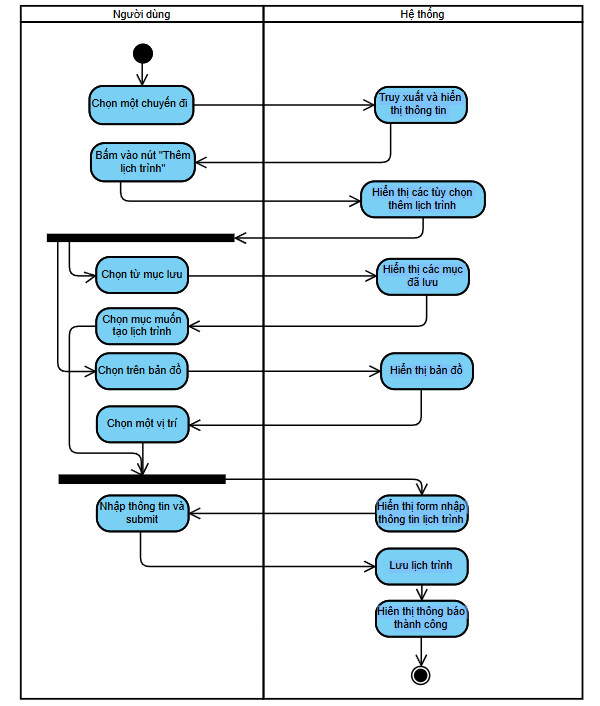
\includegraphics[width=0.5\linewidth]{figures/c3/3-3-13-ad.png} % Specified width
        &
        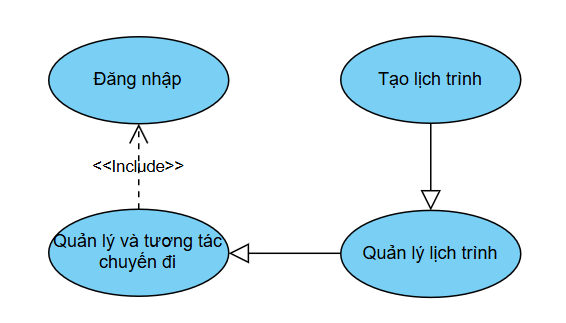
\includegraphics[width=0.45\linewidth]{figures/c3/3-3-13-rd.png} \\ % Specified width
        \hline
    \end{tabular}
\end{table}

\begin{figure}[H]
    \centering
    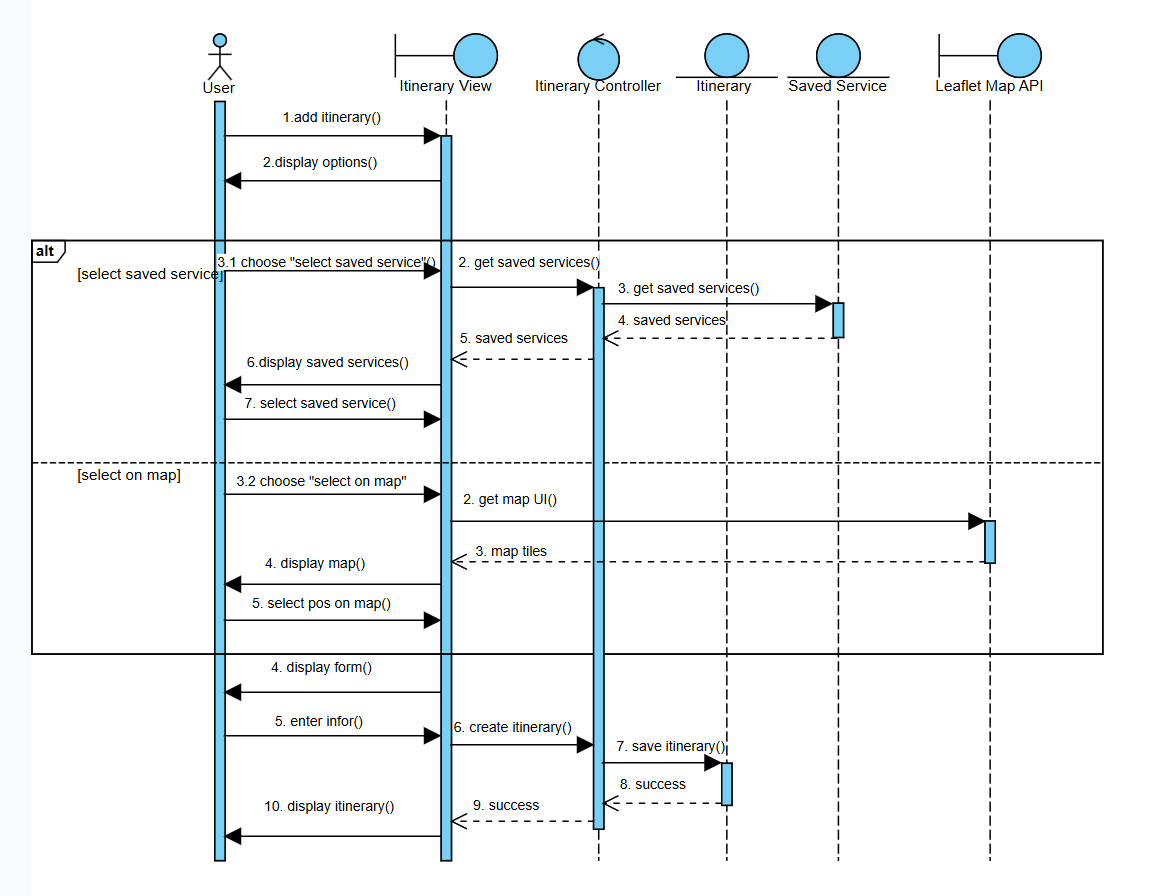
\includegraphics[width=1\textwidth]{figures/c3/3-3-13-sd.png} % Specified width
    \caption{Biểu đồ tuần tự ca sử dụng tạo lịch trình cho chuyến đi.} % (no period)
    \label{fig:3-3-13-sequence-diagram}
\end{figure}